\documentclass[11pt, oneside]{article}    % use "amsart" instead of "article" for AMSLaTeX format
\usepackage{geometry}                   % See geometry.pdf to learn the layout options. There are lots.
\geometry{letterpaper}                      % ... or a4paper or a5paper or ... 
%\geometry{landscape}                   % Activate for for rotated page geometry
\usepackage[parfill]{parskip}       % Activate to begin paragraphs with an empty line rather than an indent
\usepackage{graphicx}       % Use pdf, png, jpg, or eps§ with pdflatex; use eps in DVI mode
                % TeX will automatically convert eps --> pdf in pdflatex  
                
\setlength{\topmargin}{-0.5in}
\setlength{\textheight}{9in}
\setlength{\textwidth}{7in}
\setlength{\oddsidemargin}{-.25in}

\title{Assignment 2: Multilayer Neural Networks}
\author{Ryan Bernstein}
%\date{}

\begin{document}
\maketitle

Each experiment was run with a limit of 100 epochs.

\section*{Experiment 1: Control}

\begin{center}
	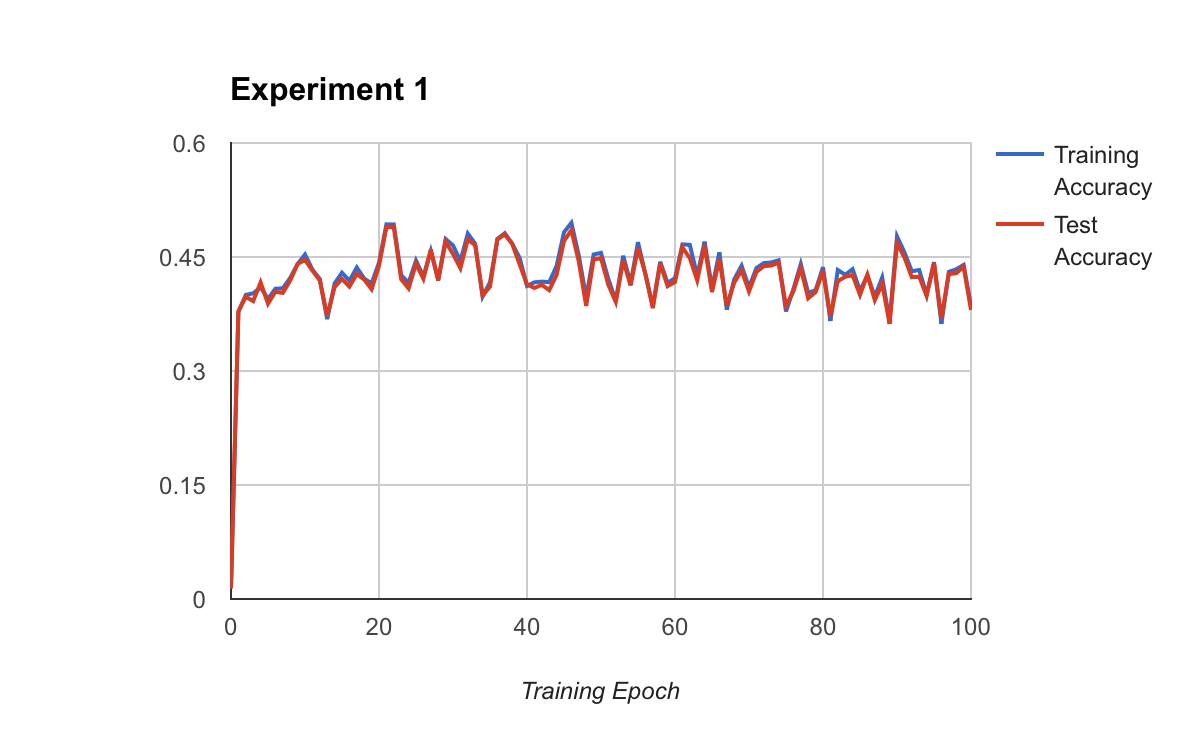
\includegraphics[width=6in]{Exp1}
\end{center}

There doesn't appear to be evidence of overfitting. While both training and test accuracies vary after an initial spike, they don't diverge significantly. In the event of overfitting, we'd expect the training accuracy to be much higher than the test accuracy.

\section*{Experiment 2: Effects of Varying Learning Rate}

\begin{center}
	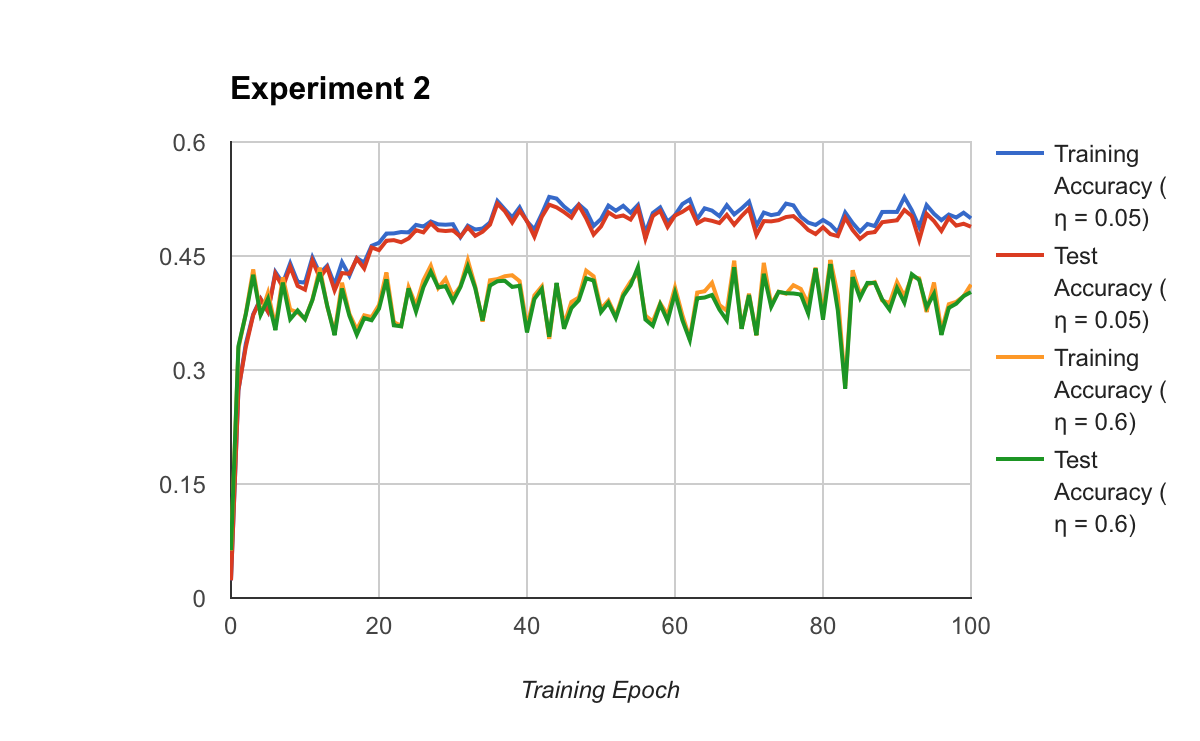
\includegraphics[width=6in]{Exp2}
\end{center}

Low learning rates seem to result in higher training and test accuracies than do high ones. In neither case do we see evidence of overfitting. The tests with the lower learning rate have higher overall accuracies than do the control tests, whereas the accuracies from the tests with higher learning rates are lower.

\section*{Experiment 3: Effects of Varying Momentum}

\begin{center}
	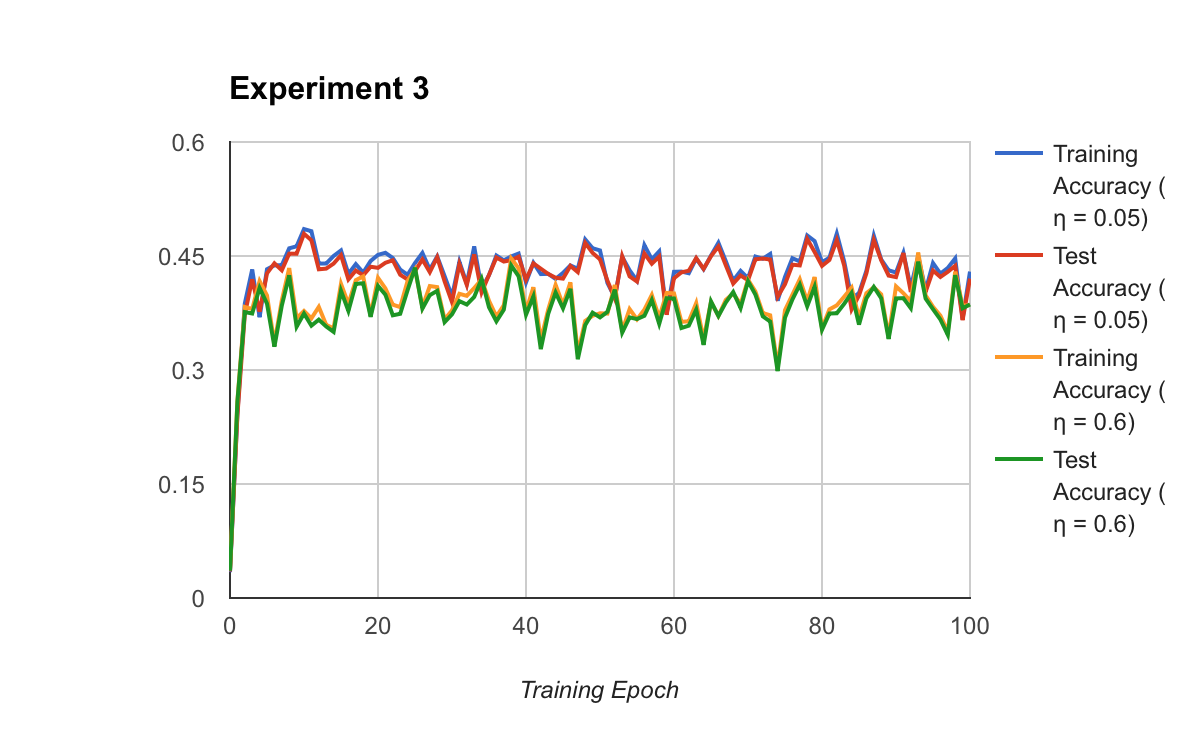
\includegraphics[width=6in]{Exp3}
\end{center}

Notably, the experiments with low momentum appear to center around ~45\% accuracy, which is similar to the control. Raising the momentum to 0.6 causes a decrease in accuracy, rather than lowering the momentum to 0.05 causing a significant increase.

\section*{Experiment 4: Effects of Varying Hidden Layer Width}

\begin{center}
	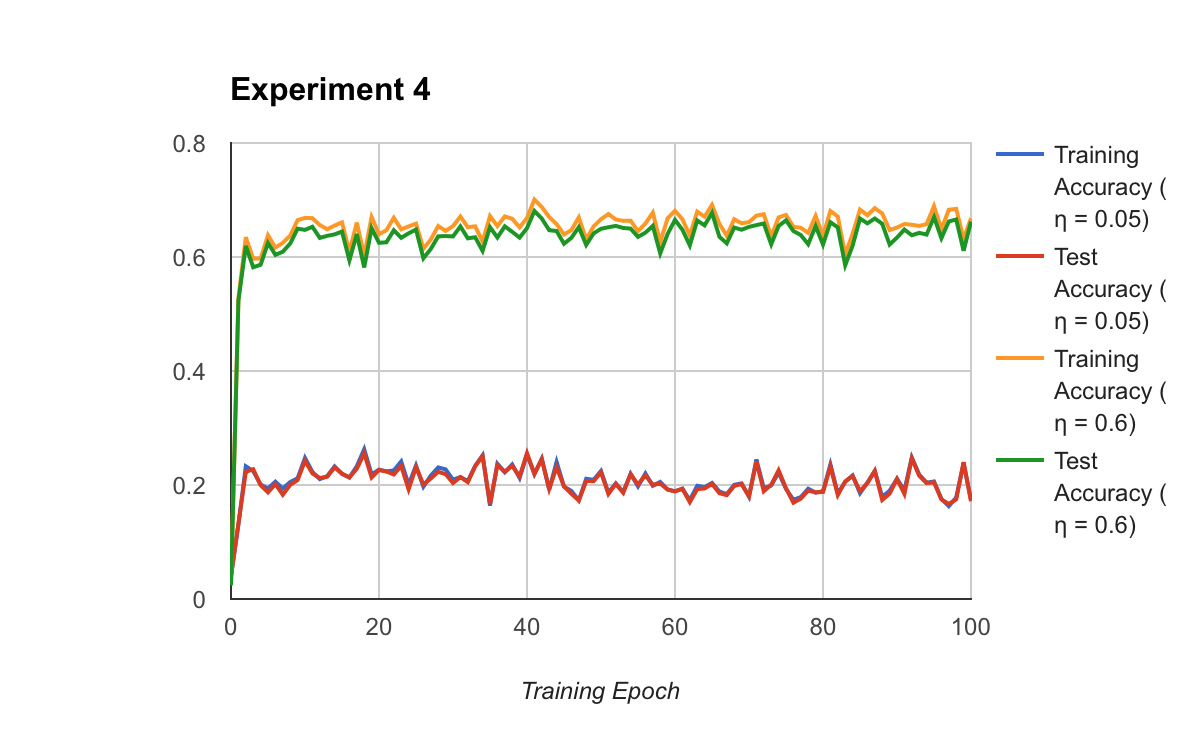
\includegraphics[width=6in]{Exp4}
\end{center}

Here we see our highest divergence yet. The width of the hidden layer appears to make the largest difference in overall accuracy. While we've heard that widening the hidden layer can lead to overfitting, it seems that 8 hidden nodes is not enough to cause this phenomenon.

\end{document}